
%(BEGIN_QUESTION)
% Copyright 2007, Tony R. Kuphaldt, released under the Creative Commons Attribution License (v 1.0)
% This means you may do almost anything with this work of mine, so long as you give me proper credit

Working on a boiler commissioning project, you are tasked with tuning the feedwater controls, documented in this functional diagram:

$$\includegraphics[width=15.5cm]{i01800x01.eps}$$

In what order would you calibrate and/or tune the following components of this control system, and why?

\begin{itemize}
\item{} Steam flow transmitter
\item{} Feedwater flow transmitter
\item{} Level transmitter
\item{} Level controller
\item{} Feedforward summer (bias and gains)
\item{} Flow controller
\end{itemize}

Describe how you would safely tune the two controllers with the boiler operating.  In other words, how would you recommend everything be set up so as to tune one controller at a time with a minimum of upset to the boiler?  Also, qualitatively propose the PID constant values needed by each controller (e.g. ``aggressive integral action,'' etc.).

\underbar{file i01800}
%(END_QUESTION)





%(BEGIN_ANSWER)

First, the transmitters may be calibrated at any time, even if the boiler is not ready to run, since all that is required is a bench calibration with instrument air.

\vskip 10pt

For tuning purposes, the boiler should be started in manual mode and given a constant load (venting steam).  The first controller to tune should be the flow controller.  The next should be the level controller.  Finally, the summer gains and biases should be adjusted.  I'll let you describe how and why for each controller, and also estimate the PID values!

%(END_ANSWER)





%(BEGIN_NOTES)

The feedwater flow controller should be tuned first because it is the slave loop in a cascade system.  It should operate predominantly on integral control, being a fast self-regulating process.

The steam drum level controller comes next, being the master in a cascade system.  Normally, a liquid level controller should control predominantly on proportional action, but it would be good to moderate the gain on this controller to avoid problems associated with boiler shrink and swell.  Try a gain of 1 (100\% proportional band) and enough integral to take care of offset.

Finally, once the flow and level controllers have been tuned, it is time to adjust the settings inside the feedforward summer.  Proper adjustments here can only be made in response to changes in load, so you will need to adjust the steam vent valve from time to time to check process response.

%INDEX% Control, PID tuning: proper sequence for three-element boiler level controls
%INDEX% Process: boiler feedwater control

%(END_NOTES)


